\documentclass[a4paper,11pt,oneside,openany]{jsbook}
%
\usepackage{amsmath,amssymb}
\usepackage{bm}
\usepackage{graphicx}
\usepackage{subfigure}
\usepackage{verbatim}
\usepackage{wrapfig}
\usepackage{ascmac}
\usepackage{makeidx}
%
\makeindex
%
\setlength{\textwidth}{\fullwidth}
\setlength{\textheight}{40\baselineskip}
\addtolength{\textheight}{\topskip}
\setlength{\voffset}{-0.55in}
%
\newcommand{\diff}{\mathrm{d}}  %微分記号
\newcommand{\divergence}{\mathrm{div}\,}  %ダイバージェンス
\newcommand{\grad}{\mathrm{grad}\,}  %グラディエント
\newcommand{\rot}{\mathrm{rot}\,}  %ローテーション
%
\title{PHP MasterBook}
\author{Piffett}
\date{\today}
\begin{document}
%
%
\maketitle
%
%
\frontmatter
%
\addcontentsline{toc}{chapter}{概要}
\chapter*{概要}

この本はProgateやPaizaやdotinstallをやって、なんとなくフレームワークとかも使えるようにはなったけど、フレームワークが何しているのかわからない!というような人に向けて、Webアプリを作りながら少しずつWebに関係する様々な技術や考え方を学んでいきます。
 
\section*{なぜこの本を書くのか}

昨今のプログラミングブームによって、プログラミング言語やフレームワークを道具として使うための教材は豊富に揃ってきました。しかし、2000年代と違いWeb開発の難易度は大きく上がりました。Laravelのような重厚なフレームワークが台頭し、AWSを始めとするクラウドサービスも普及し、これらのサービスを使いこなすことが必要不可欠になりました。また、GitやDockerのようなツールを使えることがWebエンジニアのリテラシーとなり、より一層Web開発の基礎知識を学ぶことが難しくなってきました。この教材は最初に生PHPでアプリケーションを作りながら徐々に抽象化していって、小さなフレームワークを作っていきます。その過程の中で、現在のフレームワークがどのような思想で作られているかを学びます。

\section*{PHPで学ぶ理由}

PHPはWeb開発を行うのに特化した言語です。多くのプログラミング言語の場合、小さなWebアプリケーションを開発する場合でも複数のライブラリを導入する必要がありますが、PHPの場合は必要ありません。また、徳丸本など、Webに関連する技術をPHPで説明するケースも多いため、PHPを採用しています。


\tableofcontents
%
%
\mainmatter
%
\chapter{基礎知識と環境構築}

この章ではWebの中核をなすLAMPと呼ばれる概念を説明しながら、環境構築を行います。LAMPが何の頭文字か分かる方や、Dockerなど環境構築に慣れている方はこの章を読み飛ばして各自環境構築していただいて構いません。

\section{LAMPとは}

LAMPとはWebアプリケーションを作成する上で使われる、「Linux、Apache、MySQL、PHP」の四つをまとめたワードです。いまではApacheがNginxになったり、MySQLがPostgreSQLになったり、PHPがRubyだったりPythonになったりしますが、基本的な構成要素は大きく変わっていません。

\begin{center}

\includegraphics[width=10cm]{./chap1_fig/LAMP.png}

LAMPのそれぞれのソフトウェアのロゴ
\end{center}

\subsection{避けては通れないOS、Linux}

いまこの教材を読んでいるあなたはおそらく何らかのOSが載っているデバイスを使っていることでしょう。WindowsだったりMacOSであったりAndroidだったりするでしょう。もしプログラミングを真面目にやっていくならば、Linuxは避けては通れないOSです。LinuxはLinus TorvaldsがUNIXと呼ばれるOSをベースに開発されたOSです。オープンソースでプログラムの中身が公開されており、使用するのにお金がかからないので多くの電子機器で利用されています。先ほど述べたAndroidもLinuxをベースに作られています。DockerはLinuxの上で動作しますし、組み込みでもLinuxが標準的なOSになりつつあります。Linuxを避けてプログラミングをするのはもう難しいでしょう。

\subsection{WebサーバーのApache}

Webサーバーです。インターネットでの情報はバケツリレーです。自分勝手にデータを投げつけてもだれも回してくれません。どのように接続を確立してどんな形でデータを送るかの約束事を「プロトコル」と言います。Webサービスにおいては、HTTPと呼ばれるプロトコルでデータを送受信します。最近ではデータを暗号化して、バケツリレーの途中でデータが盗まれないようにしたHTTPSがよく用いられています。Apacheはこのようなプロトコルから暗号化されたデータを復号したり、取り出したデータをPHPに渡す役割をしています。

また、最近ではNginxと呼ばれるWebサーバーが用いられるようになりました。Apacheと違い、送られたデータを別の場所に中継するリバースプロキシや、送られたデータを二台以上のサーバーに分散させるロードバランサーといった機能が搭載されています。

\subsection{データベースのMySQL}

やっぱりデータを保存できなければ面白くありません。自分のツイートしかみれないTwitterは面白くないですよね?ユーザーから送信されたデータを保存するために使われるソフトウェアがデータベースです。もちろんデータをテキストファイルに保存しても問題ありません。しかし、ある日付だけ取り出したいだとか、もしコンピューターが一台壊れてもデータが消えないようにしたいだとか、そういうことを考えると全部自分でシステムをくみ上げるのは途方もない作業になります。そこでデータベースにデータを保存しておくことで、このような問題を解決します。データベースは自分の書いたプログラムからSQLと呼ばれる言語で命令を送って操作します。SQLの命令はPHPで作ってもPythonで作っても全く同じようにデータベースは動作します。なので、PHPでwebサービスを動かしながら、裏でPythonを使ってデータ分析をする、みたいな使い方をすることもできます。

\subsection{プログラミング言語のPHP}

これから学んでいくプログラミング言語です。以下の特徴があります。

\begin{itemize}
  \item HTMLに埋め込むような書き方ができる
  \item 動的型付け言語
  \item Webアプリ向けの豊富な組み込み関数
  \item Webアプリを作るうえで使われるフレームワークが豊富
\end{itemize}

\section{環境構築}

さて、これから最も難しいとされる環境構築です。すでにDockerなど使い慣れている環境があればそれを用いてください。今回はPaizaCloudを用いて環境構築をします。

\begin{center}
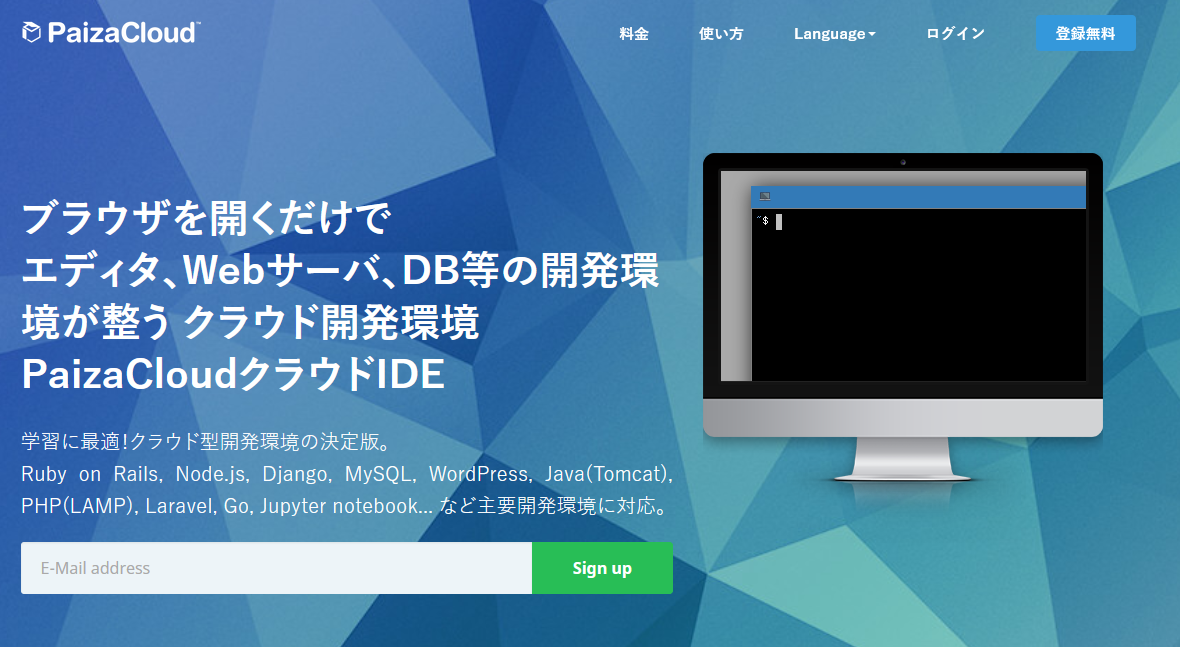
\includegraphics[width=10cm]{./chap1_fig/paizacloud.png}

オンライン開発環境のPaizaCloud
\end{center}

まずはアカウント登録してログインしましょう。そしたら以下の画面が出てくると思います。「新規サーバーを作成」をクリックしましょう。

\begin{center}
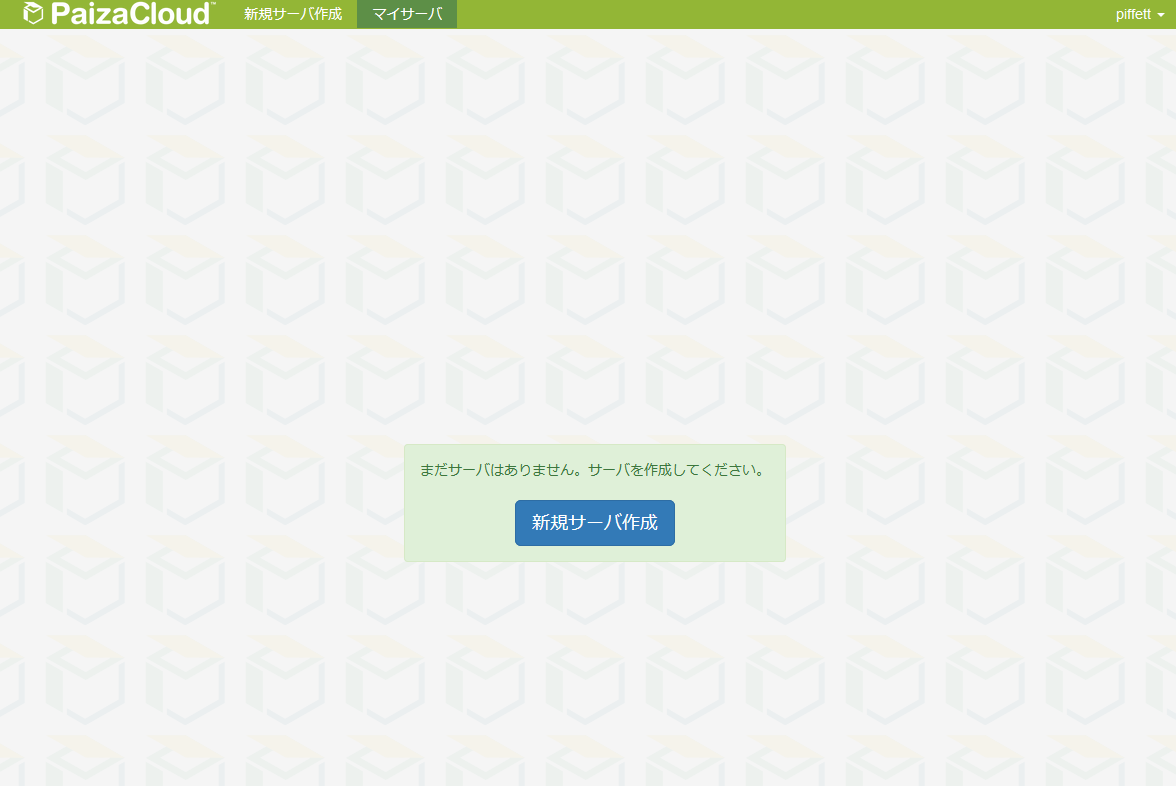
\includegraphics[width=10cm]{./chap1_fig/paiza1.png}

ログインして最初に出る画面
\end{center}

そしたら以下のように画面が出てきているので、ハイライトされている部分を同じようにクリックして設定しましょう。LAMPのPHP, MySQL, Apacheがあるのが分かると思います。

\begin{center}
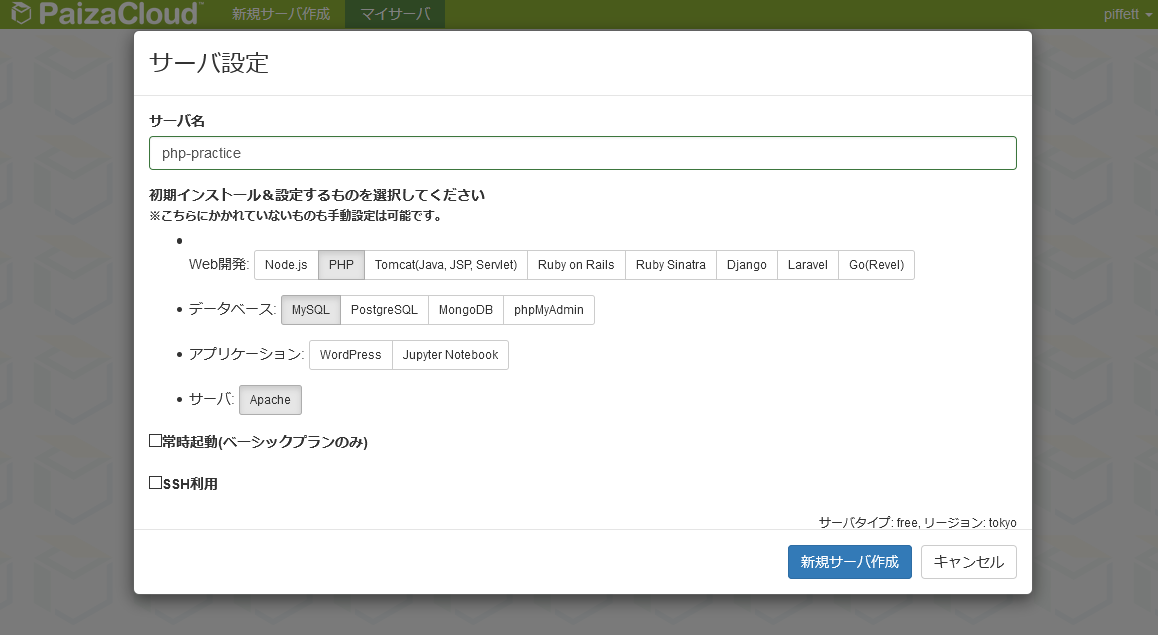
\includegraphics[width=10cm]{./chap1_fig/paiza2.png}

LAMP環境を作るサーバ設定
\end{center}

しばらくすると以下のような画面が出てきます。このような画面が出てくれば成功です。

\begin{center}
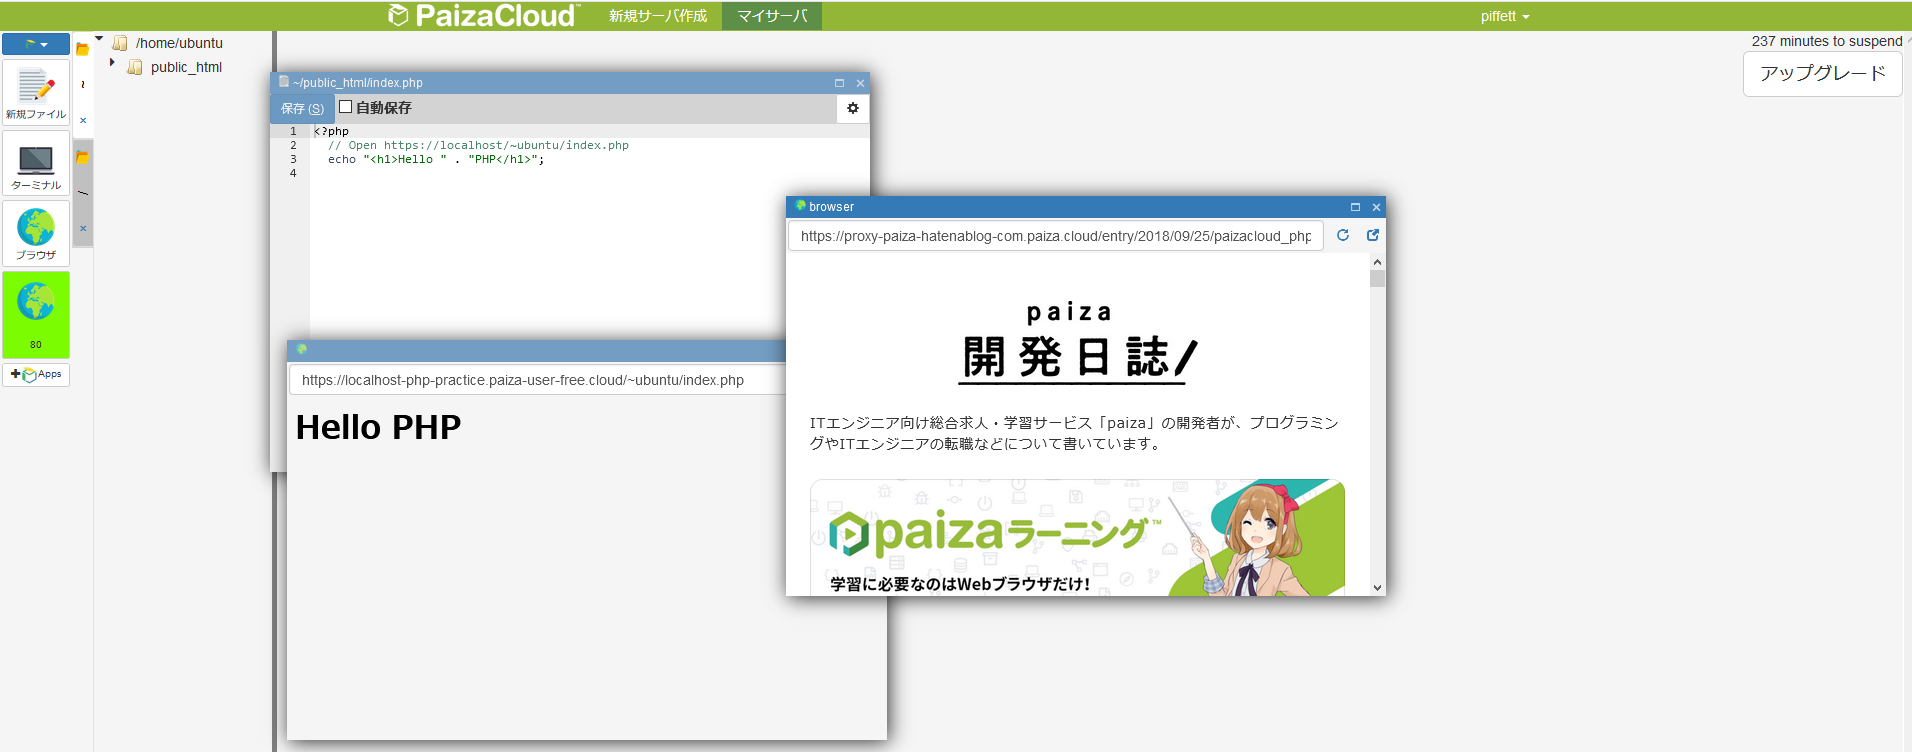
\includegraphics[width=13cm]{./chap1_fig/paiza3.png}

LAMP環境が整った状態
\end{center}




bbbb
%
%
\appendix
%
あぺA
\include{appendixB}
%
%
\chapter*{謝辞}
\addcontentsline{toc}{chapter}{謝辞}

ありがとーー!
%
%
長谷川泰広(@Piffett)

東京理科大学基礎工学部電子応用工学科
%
%
\newpage
\printindex
%
%
\end{document}